\documentclass[../main.tex]{subfiles}


\begin{document}
	\subsection{Операторное разложение единицы. Корневые подпространства.}
	\begin{minipage}{0.5\textwidth}
		$\phi(t) = \prod\limits_\lambda (t-\lambda)^{m(\lambda)}$
	\end{minipage}
	\begin{minipage}{0.5\textwidth}
		$\sum\limits_\lambda m(\lambda) = m\\
		deg \ \phi = m$
	\end{minipage}\\
	$P_{m-1}$ -- линейное пространство многочленов степени не выше $m-1\\
	dimP_{m-1} = m\\
	\phi(t) = \underset{\overset{\mathlarger{\nwarrow \nearrow}}{\text{вз. просты}}}{(t-\lambda)^{m(\lambda)}\phi_\lambda(t)} \ \ \; 
	\begin{matrix}
	\phi_\lambda(t) = \prod\limits_{\mu\neq \lambda} (t-\mu)^{m(\mu)}\\
	\phi_\lambda(\lambda) \neq 0\\
	\phi_\lambda(\mu) = 0\\
	\mu \neq \lambda
	\end{matrix}$
	\begin{defin}
		$I_\lambda = \{p\in P_{m-1} | p\vdots \phi_\lambda\}$\\
		\textbf{Главный идеал}, порожденный многочленом $\phi_\lambda = \\
		= \{f\in P_{m(\lambda)-1}|p = f_\lambda \phi_\lambda  \}\\
		I_\lambda$ -- линейное подпространство $P_{m-1}\\
		p_{1, 2}\vdots \phi_\lambda \Rightarrow (p_1 + \alpha p_2)\vdots\phi_\lambda$
	\end{defin}
	\begin{theorem}
		$P_{m-1} = \bigoplus\limits_\lambda I_\lambda$
	\end{theorem}
	\begin{proof}\
		\begin{mylist}
			\item Дизъюнктность.\\
			$\0 = \sum\limits_\lambda \underbrace{f_\lambda\phi_\lambda}_{\in I_\lambda}  = 
			f_\lambda\cdot \phi_\lambda + \underbrace{\sum\limits_{\mu\neq \lambda}f_\mu \underbrace{\phi_\mu}_{\vdots (t-\lambda)^{m(\lambda)}}}_{\vdots (t-\lambda)^{m(\lambda)}}\\
			\Rightarrow f_\lambda \cdot \underset{\text{вз. просты}}{\phi_\lambda \vdots (t-\lambda)^{m(\lambda)}} \Rightarrow \underset{\stackrel{\uparrow}{deg \ f_\lambda = m(\lambda)-1}}{f_\lambda} \vdots (t-\lambda)^{m(\lambda)} \Rightarrow f_\lambda \equiv 0 \\
			\Rightarrow \forall \lambda \ \ \ f_\lambda \equiv 0 \Rightarrow f_\lambda \phi_\lambda \equiv \0 \Rightarrow \text{Дизъюнктны}$
			\item
			\belowbaseline[-12pt]{
				$\begin{array}{lcl}
				dim P_{m-1} & = & m\\
				|| & & \\
				\sum\limits_\lambda dim I_\lambda & = & \sum\limits_\lambda m(\lambda) = m
				\end{array}$}\\\\
			$I_\lambda \subset P_{m-1}\\
			\\
			\Rightarrow P_{m-1} = \bigoplus\limits_\lambda I_\lambda$
		\end{mylist}
	\end{proof}
	\begin{corollary}
		$\forall p \in P_{m-1} \ \exists! \ p = \sum\limits_\lambda p_\lambda\\
		p_\lambda \in I_\lambda\\
		\boxed{1 = \sum\limits_\lambda p_\lambda\text{ -- полиномиальное разложение единицы}}$ 
	\end{corollary}
	\newpage
	\begin{remark} \
		\begin{mylist}
			\item 
			$\lambda \neq \mu\\
			\begin{array}{rclcl}
			p_\lambda & \cdot & p_\mu & \vdots & \phi\\
			|| & & || & &\\
			f_\lambda\phi_\lambda & & f_\mu\phi_\lambda & = & \eta \cdot \phi\\
			& & \uparrow & & \\
			& & (t-\lambda)^{m(\lambda)} & &
			\end{array}$
			\item $\forall \lambda \ m(\lambda) = 1$\\
			\textbf{Если.} Т. е. все корни $\phi$ взаимно простые.\\
			$f_\lambda = const \ \ \ (def \ f_\lambda = m(\lambda) - 1 = 0)$
		\end{mylist}
	\end{remark}
	\begin{theorem}[Лагранжа] \ \\
		$\forall \lambda: m(\lambda) = 1 \Rightarrow \\
		\forall p \in P_{m-1} \ \ p(t) = \sum\limits_\lambda \frac{p(\lambda)}{\phi'(\lambda)}\cdot \phi_\lambda(t)$
	\end{theorem}
	\begin{proof}\ \\
		$\text{корень }\phi \rightarrow \mu \neq \lambda \ \ \begin{matrix}
			\phi_\lambda(\mu) = 0\\
			\phi_\lambda(\lambda) \neq 0
		\end{matrix}\\
		p(t) \ \sum\limits_\lambda p_\lambda(t) = $\belowbaseline[-12pt]{$\begin{array}{rcl}
			\sum\limits_\mu
			& \underset{\uparrow}{\boxed{f_\mu}} & \cdot\; \phi_\mu(t)\\
			\multicolumn{3}{c}{\begin{matrix}
				const,\text{ т.к. }\\
				\text{корни взаимно}\\
				\text{просты}
			\end{matrix}}
		\end{array}$}\\
		$p(\lambda) = f_\lambda \cdot \phi_\lambda(\lambda)
		\Rightarrow \forall \lambda : f_\lambda = \frac{p(\lambda)}{\phi_\lambda(\lambda)}\\
		\phi(t) = \prod\limits_\mu (t-\mu)\\
		\phi'(t) = \sum\limits_\mu \underbracket{\prod\limits_{\lambda\neq \mu} (t-\lambda)}_{\phi_\mu(t)} = 
		\sum\limits_\mu \phi_\mu(t)\\
		\phi'(\lambda) = \sum\limits_\mu$ \belowbaseline[-12pt]{$\begin{array}{cl}
			\phi_\mu(\lambda) & = \phi_\lambda(\lambda)\\
			\mathsmaller{||} & 
			\\ \mathsmaller{0 \; \mu \neq \lambda} & 
		\end{array}$} $
		\Rightarrow f_\lambda = \mathlarger{\frac{p(\lambda)}{\phi'(\lambda)}}
		\Rightarrow p = \sum\limits_\lambda \mathlarger{\frac{p(\lambda)}{\phi'(\lambda)}} \phi_\lambda(t)$
	\end{proof}
	\begin{corollary}
		$\forall \lambda: m(\lambda) = 1\\
		1 = \sum\limits_\lambda p_\lambda \Rightarrow \boxed{t = \sum\limits_\lambda \lambda p_\lambda}$
	\end{corollary}
	\begin{proof}
		По теореме: $1 = \sum\limits_\lambda \boldsymbol{p_\lambda} = \sum\limits_\lambda f_\lambda \cdot \phi_\lambda = \sum\limits_\lambda \mathlarger{\frac{1}{\boldsymbol{\phi'(\lambda)}}} \cdot \boldsymbol{\phi_\lambda(t)}$\\
		По теореме: $t = \sum\limits_\lambda \mathlarger{\frac{\lambda}{\boldsymbol{\phi'(\lambda)}}}\boldsymbol{\phi_\lambda(t)} = \sum\limits_\lambda \lambda p_\lambda$
	\end{proof}\ \\
	$\A \in End(V)\\
	\phi$ минималный многочлен, все корни $\in K (\Rightarrow \text{ все корни }\chi \in K \\
	\Rightarrow \text{т.е. все с.ч. }\in K \text{ -- I, II случаи})\\
	1 = \sum\limits_{\lambda} p_\lambda(t)$\\
	\begin{minipage}{0.2\textwidth}
		$\p_\lambda:=p_\lambda(\A)\\
		\p_\lambda\in End(V)\\
		\p_\lambda$ -- проекторы $?$
	\end{minipage}
	\begin{minipage}{0.6\textwidth}
		$
		\boxed{\E = \sum\limits_\lambda \p_\lambda}$ операторное разложение единицы\\
		$\uparrow$ это уже есть
	\end{minipage}\\\\
	Достаточно проверить $\underset{\lambda\neq \mu}{\p_\lambda \cdot \p_\mu} = \0\\
	\p_\lambda = p_\lambda(\A) = \underset{\nwarrow \nearrow}{f_\lambda(\A)\cdot \phi_\lambda(\A)}\\
	\lambda\neq \mu\\
	\p_\mu = p_\mu(\A) = \underset{\nwarrow\nearrow}{f_\mu(\A)\cdot\phi_\mu(\A)}\\
	\text{перестановочны, т.к. многочлены от }\A\\\\
	\begin{array}{llr}
		\multicolumn{3}{l}{
			\p_\lambda\p_\mu = f_\lambda(\A)\cdot f_\mu(\A) \underset{\mathlarger{\uparrow}}
			{\phi_\lambda(\A)} \cdot \boldsymbol{\phi_\mu(\A)} = \0
		}\\
	\updownarrow & \text{содержит}&\\
	(p_\lambda \cdot p_\mu \vdots \phi \text{ см. замеч. 1}) & \eta(\A)\boldsymbol{(t-\mu)^{m(\mu)}} & \phi(\A) = \0
	\end{array}\\\\
	\Rightarrow \p_\lambda $ проекторы -- \textbf{спектральные проекторы $\A$}\\
	$Im\p_\lambda$ \textbf{спектральное подпространство}\\
	$\underset{7.5}{\Rightarrow} \boxed{V = \bigoplus\limits_\lambda Im\p_\lambda}$
	\begin{examples}
		$A = \begin{pmatrix}
			1 & -3 & 4\\
			4 & -7 & 8\\
			6 & -7 & 7
		\end{pmatrix} \begin{matrix}
			\lambda_1 = -1 & \alpha(\lambda_1) = 2\\
			\lambda_2 = 3 & \alpha(\lambda_2) = 1
		\end{matrix}\\
		V_{\lambda_1} = span\begin{pmatrix}
			1\\2\\1
		\end{pmatrix} \ \ \ \; \gamma(\lambda_1) = 1 < \alpha(\lambda_1) \Rightarrow \text{ не о.п.с.}\\
		V_{\lambda_2} = span\begin{pmatrix}
			1\\2\\2
		\end{pmatrix} \ \ \ \; \gamma(\lambda_2) = 1\\
		\chi(t) = -(t+1)^2(t-3) \quad \phi_{\lambda_1} = (t-3)\\
		\phi(t) = (t+1)^2(t-3) \quad \phi_{\lambda_2} = (t+1)^2\\
		1 = \sum\limits_\lambda p_\lambda = p_{\lambda_1} + p_{\lambda_2} = f_{\lambda_1}\phi_{\lambda_1} 
		+ f_{\lambda_2}\cdot\phi_{\lambda_2} =\\
		= f_{\lambda_1}(t-3) + f_{\lambda_2}(t+1)^2\\
		\text{Прав. дробь }\mathlarger{\frac{1}{\phi}} = \sum\limits_\lambda \underset{\text{Правильн.}}{\mathlarger{\frac{f_\lambda \cdot \phi_\lambda}{\phi}}} = \sum\limits_\lambda \underset{\text{Правильн. дробь}}{\mathlarger{\frac{f_\lambda}{(t-\lambda)^{m(\lambda)}}}}\\
		deg \ f_\lambda < m(\lambda)\\
		\mathlarger{
			\frac{1}{(t+1)^2(t-3)} = \underset{\text{простейшие}}{\frac{A_1}{t+1} + \frac{A_2}{(t+1)^2}} + 
			\frac{A_3}{t-3} = \frac{-\frac{1}{16}t - \frac{5}{16}}{(t+1)^2} + \frac{\frac{1}{15}}{t-3}
		}\\
		1 = \underbracket{(-\frac{1}{16}t - \frac{5}{16})\overbrace{(t-3)}^{\phi_\lambda}}_{p_{\lambda_1}} + 
		\underbracket{\frac{1}{15} \overbrace{(t+1)^2}^{\phi_{\lambda_2}}}_{p_{\lambda_2}}\\
		\p_1 = p_{\lambda_1}(A) = \begin{pmatrix}
			0 & 1 & -1\\
			-2 & 3 & -2\\
			-2 & 2& -1
		\end{pmatrix} \; p_1 + p_2 = E\\
		\p_2 = p_{\lambda_2}(A) = \begin{pmatrix}
			1 & -1 & 1\\
			2 & -2 & 2\\
			2 & -2 & 2
		\end{pmatrix}
		$
	\end{examples}
	\begin{remark}
		$\forall \lambda: m(\lambda) = 1$\\
		Из следствия теоремы Лагранжа $t = \sum\limits_\lambda \lambda p_\lambda\\
		\boxed{\A = \sum\limits_\lambda \lambda \p_\lambda}  \nearrow \; \quad 1 = \sum p_\lambda \; \; $ 
		спектральное разложение о.п.с.\\\\
		$\boxed{\A \text{ о.п.с.} \Leftrightarrow \forall \lambda: m(\lambda) = 1
		\text{     \ \ \ \ \; Доказательство позже}}$
	\end{remark}
	\begin{defin}
		$K_\lambda = Ker(\A - \lambda\E)^{m(\lambda)}$\\
		называется \textbf{корневым подпространством }$\A$
	\end{defin}
	\begin{theorem}\
		\begin{mylist}
			\item 
			$K_\lambda$ инвариантно относительно $\A$
			\item $Im \p_\lambda = K_\lambda$
			\item $(t-\lambda)^{m(\lambda)}$ минимальный многочлен $\A|_{K_\lambda = Im\p_\lambda}$
		\end{mylist}
		$\Rightarrow \boxed{V = \bigoplus\limits_\lambda K_\lambda}$
	\end{theorem}
	\begin{proof}\
		\begin{mylist}
			\item 
			$x\in K_\lambda \overset{?}{\Rightarrow} \A x \in K_\lambda\\
			\underset{\stackrel{\nwarrow\nearrow}{\text{перестановочны}}}{(\A-\lambda\E)^{m(\lambda)} \A x}
			= \A \underbracket{(\A-\lambda\E)^{m(\lambda)} x \in K_\lambda}_{=\0} = \0\\
			\Rightarrow
			 \A x \in Ker(\A - \lambda\E)^{m(\lambda)}$
			 \item 
			 $(\A - \lambda \E)^{m(\lambda)}\p_\lambda = (\A - \lambda\E)^{m(\lambda)} f_\lambda(\A)\phi_\lambda(\A) =\\
			 = f_\lambda(\A) \cdot \underbracket{(\A - \lambda \E)^{m(\lambda)} \phi_\lambda(\A)}_{\phi(\A)} = \0\\
			 \forall x \in V\\
			 (\A - \lambda \E)^{m(\lambda)} \underbracket{\p_\lambda x}_{\in Im\p_\lambda} = \0 \Rightarrow Im\p_\lambda \subseteq Ker(\A - \lambda\E)^{m(\lambda)} = K_\lambda$\\
			 \textbf{Обратно: } $K_\lambda \overset{?}{\subseteq} Im\p_\lambda\\
			 x\in K_\lambda\\
			 \mu \neq K_\lambda \; \p_\mu x = \underbracket{
			 	\underset{
			 		\stackrel{\nearrow}
			 		{
			 			\text{содержит }(\A-\lambda\E)^{m(\lambda)}
		 			}
		 		}
	 			{
	 				f_\mu(\A)\phi_\mu(\A)x
 				}
	 	 	}_{\eta(\A)(\A - \lambda\E)^{m(\lambda)}} = \eta(\A)\cdot \underbracket{(\A-\lambda\E)^{m(\lambda)}x\in K_\lambda}_{=\0} = \0\\
 	 		x = \E x = \sum\limits_\mu \underset{\stackrel{||}{\0 \ \mu\neq \lambda}}{\p_\mu x} = \p_\lambda x \in Im\p_\lambda \Rightarrow K_\lambda \subseteq Im\p_\lambda \\
 	 		\Rightarrow \boxed{K_\lambda = Im\p_\lambda}$\newpage
 	 		\item 
 	 		$(t-\lambda)^{m(\lambda)}$ минимальный многочлен для $\A|_{K_\lambda = Im\p_\lambda}$ $?\\
 	 		(\A - \lambda \E)^{m(\lambda)}$ аннулятор $\A|_{K_\lambda}$\\
 	 		Минимальный?\\\\
 	 		$\pu \overset{\psi}{\text{не минимальный}}\\
 	 		\psi_1 = (t-\lambda)^{m(\lambda) - 1} \; \pu \text{ это минимальный многочлен}\\
 	 		\phi_1:= (t-\lambda)^{m(\lambda) - 1}\phi_\lambda(t) = $ аннулятор $\A?\\
 	 		\underset{\mu \neq \lambda}{\phi_1(\A) \p_\mu} = (\A-\lambda\E)^{m(\lambda) - 1} \phi_\lambda(\A) f_\mu (\A) \phi_\mu (\A) = \\
 	 		= \ldots \phi_\lambda(\A) \phi_\mu(\A) = \eta(\A) \cdot \phi(\A) = \0\\
 	 		\forall x \ \phi_1(\A) \p_{\lambda}x = (\A-\lambda\E)^{m(\lambda) - 1}\phi_\lambda(\A) \p_\lambda x = \\
 	 		= \phi_\lambda(\A) \underbracket{\underbracket{(\A - \lambda\E)^{m(\lambda) - 1}}_{\psi_1(\A)}
 	 		\underbracket{\p_\lambda x}_{\in Im\p_\lambda = K_\lambda}
  		   	}_{\underset{\text{ мин. многочлен по предположению}}{\psi_1(\A|_{K_\lambda})x}} = \0\\
  	   		\phi_1(\A)\p_\lambda = \0\\
  	   		\phi_1(\A)\cdot\E = \underbracket{\phi_1(\A) \sum\limits_\mu \p_\mu}_{\phi_1(\A)\p_\lambda + \sum\limits_{\mu\neq \lambda}\phi_1(\A) \p_\mu} = \0\\
  	   		\Rightarrow \phi_1 \text{ аннулятор }\A$, но степени $< \phi\\
  	   		deg\ \phi_1 = m-1 \Rightarrow \text{противоречие мин. }\phi \Rightarrow (t-\lambda)^{m(\lambda)}$ минимальный мн-н $\A|_{K_\lambda}$
		\end{mylist}
	\end{proof}
	\begin{corollary}
		$A$ о.п.с. $\Leftrightarrow \forall \lambda: m(\lambda) = 1$
	\end{corollary}
	\begin{proof}
		$(\Rightarrow) \ \; \; \A$ о.п.с.\\
		$\phi(t) \ \prod\limits_\lambda (t-\lambda) \; \; \; $ покажем что это минимальный многочлен $\A\\
		V = \bigoplus\limits_\lambda V_\lambda$ -- собственные подпространства $\A\\
		\forall v \in V \; \exists! \ v = \sum\limits_\lambda v_\lambda, v_\lambda \in V_\lambda\\
		\phi(\A) v = \prod\limits_\lambda (\A - \lambda\E) \sum\limits_\mu v_\mu = \\
		= \sum\limits_\mu \underbracket{\prod\limits_\lambda (\A - \lambda \E)}_{\phi_\mu (\A) \cdot (\A - \mu \E)} v_\mu = \sum\limits_\mu \phi_\mu (\A)\underbracket{(\A-\mu\E)v_\mu}_{\stackrel{||}{\0}} = \0\\
		v_\mu \in V_\mu = Ker(\A-\mu\E) \nearrow\\
		\Rightarrow \phi \text{ аннулятор }\A \Rightarrow$ очевидно минимальная степень $\Rightarrow$ минимальный многочлен.\\
		$(\Leftarrow) \forall \lambda: m(\lambda) = 1\\
		\underset{\stackrel{||}{Im\p_\lambda}}{K_\lambda} = Ker(\A - \lambda\E)^1 = V_\lambda\\
		V = \bigoplus\limits_\lambda K_\lambda = \bigoplus\limits_\lambda V_\lambda \Leftrightarrow \A $ о.п.с.
	\end{proof}
	\begin{examples}\ \\
		$Im\p_1 = Ker(A - \lambda_1 E)^2 = K_{\lambda_1}\\
		Im \p_2 = Ker(A - \lambda_2 E)^2 = K_{\lambda_2}\; \; \; \quad$ --- упр.
	\end{examples}
	\subsection{Нильпотентный оператор. Разложение Жордана}
	\begin{defin}
		$\B \in End(V)$ называется \textbf{нильпотентным}, если $\phi(t) = t^\nu$\\
		Минимальный многочлен $\B$, т.е. $\B^\nu = \0$\\
		\underline{$\nu$ -- индекс нильпотентности} (мин. степерь $\B^\nu = \0$)\\\\
		$\boxed{\begin{matrix}\p^2_\lambda = \p_\lambda\\\text{Идемпотентность}\end{matrix}}\\
		\text{Степень минимального многочлена} \rightarrow \nu \leq dim V \underset{\stackrel{\uparrow}{\text{степень }\chi}}{=} n$
	\end{defin}
	\begin{stat}
		$\forall \lambda: m(\lambda) \leq dim V_\lambda$
	\end{stat}
	\begin{proof}
		$(t-\lambda)^{m(\lambda)}$ минимальный мн-н $\A|_{K_\lambda}\\
		\B_\lambda = (\A-\lambda\E)|_{k_\lambda} \Rightarrow\B_\lambda^{m(\lambda)} = (\A-\lambda\E)^{m(\lambda)}|_{K_\lambda} = \0 \\
		\Rightarrow m(\lambda)$ индекс нильпотентности $\B_\lambda\in End(K_\lambda)\\
		m(\lambda) \leq dim K_\lambda$
	\end{proof}
	\begin{remark}
		$\underbracket{\sum\limits_\lambda m(\lambda)}_{deg \ \phi} \leq \underset{\stackrel{||}{deg \ \chi}}
		{\sum}dimK_\lambda = n$\\
		\phantom\noindent\hspace{2.7in}$\bigoplus\limits_\lambda K_\lambda = V$
	\end{remark}
	\begin{theorem}[Разложение Жордана]
		\ \\
		$\forall \A \in End(V)$ можно представить в виде:\\
		$\A: \D + \B$, где $\D$ о.п.с.\\
		$\B$ нильпотентный, причем $\B\D = \D\B$ перестановочны
	\end{theorem}
	\begin{proof}
		$\phi$ -- минимальный многочлен $\A\\
		\E = \sum\limits_\lambda\p_\lambda$ операторн. разложение единицы\\
		$\D:= \sum\limits_\lambda \lambda\p_\lambda \; \; \; D$ о.п.с.$?\\
		V = \bigoplus\limits_\lambda Im\p_\lambda\\
		\pu v_\lambda \neq 0 \; \in Im\p_\lambda\\
		\underline{\underline{D v_\lambda}} = (\sum\limits_\mu \mu \p_\mu) v_\lambda = \sum\limits_\mu \mu \begin{array}{l}
			\hspace{10pt}0 \; \mu\neq \lambda\\
			\hspace{10pt}|| \\
			(\p_\mu v_\lambda)\\
			\p_\mu \p_\lambda = \0\\
			\lambda\neq \mu
		\end{array} = \lambda\p_\lambda v_\lambda = \dunderline{\lambda\cdot v_\lambda}\\
		\Rightarrow \lambda \text{ с.ч. }\D, v_\lambda$ соотв. с.в. $\D\\
		\Rightarrow \boxed{\begin{matrix}
				Im\p_\lambda\subseteq V^\D_\lambda \text{ собств. подпр-во }\D\text{, отвечающ. с.ч. }\lambda\\
				V = \bigoplus\limits_\lambda Im\p_\lambda \text{ дизъюнктны}
			\end{matrix}} \Rightarrow Im\p_\lambda = V^\D_\lambda$\\\\
		Объединение базисов $Im\p_\lambda = $ базис $V$\\
		Каждый вектор из $Im\p_\lambda$ -- это с.в. $\D\\
		\Rightarrow$ у $V$  есть базис из с.в. $\Leftrightarrow D$ о.п.с.\\
		$\B = \A - \D = \A \E - \sum\limits_\lambda \lambda \p_\lambda = \A \sum\limits_\lambda \p_\lambda - \sum\limits_\lambda \lambda\p_\lambda = \sum\limits_\lambda (\A -\lambda\E) \p_\lambda \ns
		\nu = \underset{\lambda}{max}\ m(\lambda) \; \underset{\text{мин. мн-н }\A}{\phi(t)} = \prod\limits_\lambda(t-\lambda)^{m(\lambda)}\nb
		\B^\nu = (\sum\limits_\lambda(\A - \lambda \E) \p_\lambda)^\nu = \sum\limits_\lambda(\A - \lambda\E) ^\nu \p_\lambda = \\
		\phantom{se} \hspace{20pt}\begin{matrix}
			\p_\lambda \p_\mu = \0\\
			\lambda\neq \mu\\
			\p^2_\lambda = \p_\lambda
		\end{matrix}\n
		= \sum\limits_\lambda \underset{\stackrel{\nwarrow \nearrow}{\text{все операторы перестановочны}}}
		{(\A - \lambda \E)^\nu \underbracket{f_\lambda (\A) \phi_\lambda (\A)}_{\p_\lambda}} = \n
		\sum\limits_\lambda(\A - \lambda\E)^{\nu - m(\lambda)} f_\lambda(\A) \cdot \underbracket{(\A - \lambda\E)^{m(\lambda)} \phi_\lambda (\A)}_{\phi(\A) = \0} = 0\\
		\phantom{}\hspace{200pt}\B \text{ нильпотент}\\
		\B = \sum\limits_\lambda\underset{\stackrel{\nwarrow\nearrow}{\text{перестановочны}}}{(\A - \lambda\E)\p}\n
		D = \sum\limits_\mu \mu \p_\mu\n
		\D\B = \B\D
		$
	\end{proof}
	\begin{remark}\
		\begin{mylist}
			\item $\B = \sum\limits_\lambda(\A - \lambda\E) \p_\lambda = \sum\limits_\lambda \B_\lambda\\
			\B_\lambda = (\A-\lambda\E)|_{Im\p_\lambda = K_\lambda}$
			\item $\A, \D, \B $ все три оператора взаимно-перестановочны\\
			$\A\D = \D\A\\
			\A\B = \B\A$
		\end{mylist}
	\end{remark}
	\begin{examples}\ \\
		$A = \begin{pmatrix}
			1 & -3 & 4\\
			4 & -7 & 8\\
			5 & -7 & 5
		\end{pmatrix} \begin{matrix}
			\lambda_1 = -1\\
			\lambda_2 = 3
		\end{matrix} \; \quad\D = -1\p_1 + 3\p_2\n
		\p_1 = \begin{pmatrix}
			0 & 1 & -1\\
			-2 & 3 & -2\\
			-2 & 2 & -1
		\end{pmatrix} \ \p_2 = \begin{pmatrix}
			1 & -1 & 1\\
			2 & -2 & 2\\
			2 & -2 & 2
		\end{pmatrix}\n
		D = \begin{pmatrix}
			0 & -1 & 1\\
			2 & -3 & 2\\
			2 & -2 & 1
		\end{pmatrix} + \begin{pmatrix}
			3 & -3 & 3\\
			6 & -6 & 6\\
			6 & -6 & 6
		\end{pmatrix} = \begin{pmatrix}
			3 & -4 & 4\\
			8 & -9 & 8\\
			8 & -8 & 7
		\end{pmatrix}\n
		B = A - D = \begin{pmatrix}
			-2 & 1 & 0\\
			-4 & 2 & 0\\
			-2 & 1 & 0
		\end{pmatrix}\n
		\nu = \underset{\lambda_{1, 2}}{max} \ m(\lambda) = 2\n
		B^2 \overset{?}{=} \0 \; \quad B^2 = \begin{pmatrix}
			-2 & 1 & 0\\
			-4 & 2 & 0\\
			-2 & 1 & 0
		\end{pmatrix}\begin{pmatrix}
			-2 & 1 & 0\\
			-4 & 2 & 0\\
			-2 & 1 & 0
		\end{pmatrix} = \begin{pmatrix}
			0 & 0 & 0\\
			0 & 0 & 0\\
			0 & 0 & 0
		\end{pmatrix}\n
		\begin{pmatrix}
			1 & -3 & 4\\
			4 & -7 & 8\\
			6 & -7 & 7
		\end{pmatrix} \underset{\text{Разложение Жордана}}{=} \underset{\text{Диагонализ.}}{\begin{pmatrix}
				3 & -4 & 4\\
				8 & -9 & 8\\
				8 & -8 & 7
			\end{pmatrix}} + \underset{\text{Нильпотент.}}{\begin{pmatrix}
				-2 & 1 & 0\\
				-4 & 2 & 0\\
				-2 & 1 & 0
			\end{pmatrix}}
		$
	\end{examples}
	\begin{theorem}[Единственность разложения Жордана]\ 
		\begin{multicols}{2}
			Разложение Жордана определяется единственным образом. (Рис. 1)\\
			\begin{Figure}
				\centering
				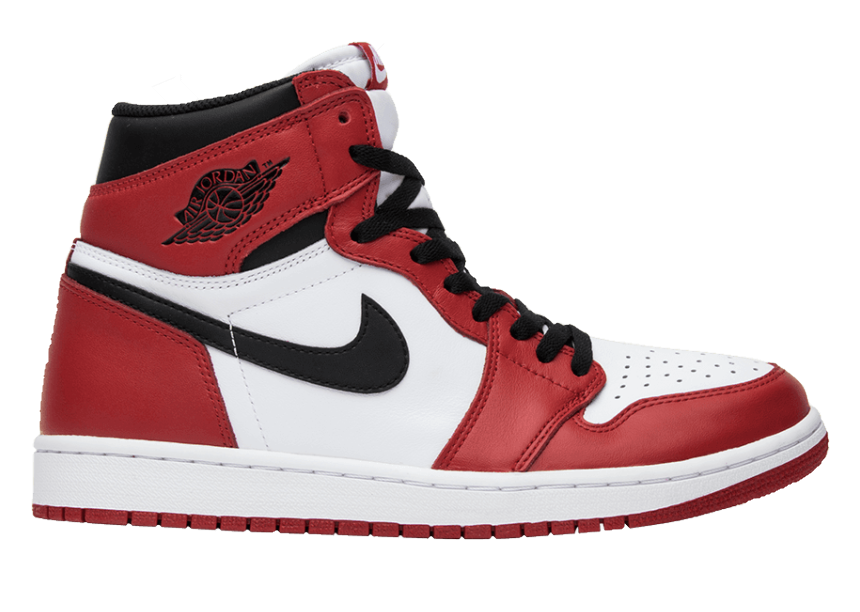
\includegraphics[width=100px]{Jordan} 
				\captionof{figure}{}
			\end{Figure}
		\end{multicols}
	\end{theorem}
	\begin{proof}
		$\pu \A = \underset{\text{о.п.с.}}{\D'} + \underset{\text{Нильпотент}}{\mathcal{C}} \; \; \; \D'
		\mathcal C = \mathcal C \D'$\n
		Т.к. $\D'$ о.п.с., то $\D' = \sum\limits_{\mu \in M} \mu Q_\mu$\n
		$M$ -- множество с.ч. $\D'\\
		Q_\mu$ спектральные проекторы\n
		$Q_\mu : V\rightarrow V^\nu_\mu\n
		\sum\limits_\mu Q_\mu = \E$\n
		\underline{Достаточно доказать: }$\D' = \D$
		\begin{mylist}
			\item Множество $M$ совпадает с множеством корней $\phi$ -- минимальн. мн-н $\A\\
			\slide{1in} \{\mu\} = \{\lambda\}$
			\item $ImQ_\mu = K_\mu \leftarrow$ корневое подпространство $\A$, отвеч. с.ч. $\mu \ (Im\p_\lambda = K_\lambda)$
		\end{mylist}
		\begin{mylist}
			\item
			$(\A - \mu\E) Q_\mu = (\sum\limits_\nu \nu Q_\nu + \mathcal C - \mu \sum\limits_\nu Q_\nu) Q_\mu 
			= \mathcal C Q_\mu\\
			\slide{1.4in} \begin{matrix}
				Q_\nu Q_\mu = 0\\
				\nu \neq \mu
			\end{matrix} \; \; \quad Q^2_\mu = Q\n
			(\A - \mu \E)^k Q_\mu$ \belowbaseline[-12pt]{$ \begin{array}{l}
					=\ \mathcal C^k Q_\mu\\
					\uparrow\\
					\text{Верно, если }\mathcal C Q_\mu = Q_\mu \mathcal C
				\end{array}$}\n
			$\Rightarrow$ докажем: $\mathcal C Q_\mu = Q_\mu \mathcal C\\
			\pu \lambda \neq \mu \; \; (\lambda-\mu) Q_\lambda \mathcal C Q_\mu = 
			\underset{Q_\lambda \D'}{(\lambda Q_\lambda)} \mathcal C Q_\mu - 
			Q_\lambda \mathcal C \underbracket{(\mu Q_\mu)}_{\D' Q_\mu} = \n
			\D' Q_\mu = \sum\limits_\lambda Q_\lambda Q_\mu = \mu Q_\mu = Q_\mu \D' \n
			Q_\lambda(\underset{\stackrel{||}{\0}}{\D'\mathcal C - \mathcal C \D'}) Q_\mu = \0$\n
			$\lambda \neq \mu \quad \quad Q_\lambda \mathcal C Q_\mu = \0 = Q_\mu \mathcal C Q_\lambda\n
			\underbrace{\sum\limits_\lambda Q_\lambda}_\E \mathcal C Q_\mu = Q_\lambda \mathcal C Q_\lambda = 
			\underset{\boxed{\E}}{\dunderline{\boxed{\sum\limits_\lambda} Q_\mu \mathcal C \boxed{Q_\lambda}}}\n
			\boxed{\mathcal C Q_\mu = Q_\mu C}\!\n
			\Rightarrow (\A -\mu \E)^k Q_\mu = \mathcal C^k Q_\mu\n
			k(\mu) = min K$, такой что $\mathcal C^k Q_\mu = \0$\n
			Такое $K(\mu)$ обязательно найдется, т.к. $\mathcal C$ -- нильпотент.\\
			$(\A - \mu \E)^{k(\mu)} Q_\mu = \0\n
			(t-\mu)^{k(\mu)}$ -- минимальный аннулятор элементов $imQ_\mu\n
			Im Q_\mu \subseteq Ker(\A - \mu\E)^{k(\mu)}$\n
			$\phi$ минимальный многочлен $\A \Rightarrow \phi(\A)$ аннулирует любые элементы $V$, \\
			в частности элементы $ImQ_\mu$\\
			Т.е. $\phi(t) $ аннулятор элементов $ImQ_\mu \Rightarrow \phi(t) \vdots (t-\mu)^{k(\mu)} \leftarrow$ 
			минимальный аннулятор для $ImQ_\mu\n
			\Rightarrow $ верно $\forall \mu \in M\n
			\psi(t) = \prod\limits_{\mu \in M} (t-\mu)^{k(\mu)} \n
			\Rightarrow \phi \vdots \psi$\n
			Покажем, что $\psi$ аннулятор $\A\\
			\psi(\A) = \psi(\A)\cdot\E = \psi(\A) \sum\limits_{\mu \in M} Q_\mu = \sum\limits_{\mu \in M}
			\prod\limits_{\nu \in M} \underset{\stackrel{\uparrow}{\text{перестановочны}}}{(\A - \nu \E)^{k(\nu)}}Q_\mu = \n
			\sum\limits_{\mu \in M} \prod\limits_{\nu \neq \mu} (\A - \nu \E)^{k(\nu)} 
			\underbracket{(\A - \mu \E)^{k(\mu)} Q_\mu}_{\stackrel{||}{\0}} = \0\n
			\Rightarrow \psi$ аннулятор $\A \Rightarrow \psi \vdots \phi$ минимальный аннулятор\\
			$\Rightarrow \psi \equiv \phi \Rightarrow \{\mu \in M\} = \{\lambda \text{ -- корни }\phi\}\n
			\slide{50pt} \begin{matrix}K(\mu) = m(\lambda)\\
			\mu = \lambda\end{matrix}$
			\item \belowbaseline[-12pt]{$
			\begin{array}{ll}
				(\A - \mu\E)^{k(\mu)} Q_\mu & = \0\\
				\slide{20pt}||\\
				(\A - \mu\E)^{m(\mu)} Q_\mu & = \0
			\end{array}$}\n
			$\mu$ корень $\phi\n
			Im Q_\mu \subseteq Ker(\A - \mu \E)^{m(\mu)} = \underset{\text{Корневое подпр-во}}{K_\mu}
			= Im\p_\mu\n
			\left.\begin{array}{ll}
				\bigoplus\limits_\mu K_\mu & = V\\
				\bigoplus\limits_\mu Im Q_\mu & = V
			\end{array}\right\} \Rightarrow Im Q_\mu = K_\mu
			\Rightarrow \D' = \D \Rightarrow \mathcal C = \B$
		\end{mylist}
	\end{proof}
	\begin{theorem}
		$\A = \D + \B$ разложение Жордана\\
		$\Rightarrow \chi_\A(t) = \chi_\D(t)$
	\end{theorem}
	\begin{proof}
		$(\chi_\A(t))^k = (det(\A-t\E))^k = det(\A - t\E)^k\n
		\B^\nu = \0\n
		\mu\text{ -- не корень   } \underset{\text{не зависит от }t}{(\chi_\A(\mu))^\nu} = 
		det((\A-\mu\E)^\nu - \underbracket{(t\B)^\nu}_{\stackrel{||}{\0}}) = \n
		= det(\underset{t = 1}{\A - \mu\E - t\B}) \cdot det(\underset{t=0}{(\A-\mu\E)^{\nu-1} + (\A - \mu\E)^{\nu-2} t \B} + \ldots + (\A - \mu\E)(t\B)^{\nu - 2} + (t\B)^{\nu - 1})$\n
		\textbf{$\mu$ -- не корень}\\
		$(\underset{\stackrel{\nparallel}{0}}{\chi_\A (\mu))^\nu}
		= det(\underset{\boxed\D}{\dunderline{\boxed\A - \mu \E \boxed{-\B}}}) \cdot
		det(\A - \mu \E)^{\nu - 1} = \n
		= \underbracket{det(\D - \mu \E)}_{\chi_\D(\mu)} \underbracket{(det(\A - \mu\E))^{\nu-1}}_{(\chi_\A(\mu))^{\nu-1}}\n
		\chi_\A(\mu) = \chi_\D(\mu)$
	\end{proof}	
	\begin{corollary}
		Если $\A = \D + \B$ разложение Жордана\n
		То $det\A = det\D$
	\end{corollary}
	\begin{proof}
		Очевидно, $\chi_\A(0) = \chi_\D(0)$
	\end{proof}
	\begin{corollary}
		$\boxed{dim K_\lambda = \alpha(\lambda)}$
	\end{corollary}
	\begin{proof}
		$\chi_\A(t) = \chi_\D(t) \Rightarrow \alpha(\lambda) = \alpha^\D(\lambda) \underset{\stackrel{\uparrow}{\text{о.п.с.}}}{=} \gamma^\D(\lambda) = dim \p_\lambda = dim K_\lambda\\
		\forall \lambda \text{ корня }\chi \text{ с.ч. (I, II)}$
	\end{proof}
	\subsection{Жорданова форма матрицы, Жорданов базис}
	$
	\begin{array}{ll}
		V = \bigoplus\limits_{\lambda \text{ с.ч.}} K_\lambda \text{ корневые } & dim K_\lambda = \alpha(\lambda)\\
		\chi(t) = \prod\limits_{\lambda\text{с.ч.}} (t-\lambda)^{\alpha(\lambda)} & \lambda \in K \text{ все корни с.ч.}\\
		\phi(t) = \prod\limits_{\lambda \text{ с.ч.}}(t-\lambda)^{m(\lambda)}
	\end{array}\n
	\begin{array}{clc}
		V_\lambda & = Ker(\A - \lambda \E) & \gamma(\lambda) = dim V_\lambda\\
		\bigcap | \\
		K_\lambda & = Ker(\A - \lambda\E)^{m(\lambda)}
	\end{array}\n
	\forall \lambda \; K_\lambda \leadsto \underset{\mathlarger{\bigcup\limits_\lambda \text{ Жорданов базис}}}{\text{ строим базис }} \leadsto $ \belowbaseline[-12pt]{$\begin{array}{l}
		\text{ матрица оператора будет иметь}\\
		\text{блочно-диагональную структуру}\\
		\text{-- Жорданова форма матрицы}
	\end{array}	
	$}\n
	$\pu K_\lambda = K \; \; \gamma(\lambda) = \gamma\\
	\alpha(\lambda) = \alpha \; \; m(\lambda) = m\n
	\B = \B_\lambda = (\A - \lambda\E)|_{K_\lambda}\; \; \quad
	dim = \gamma\n
	\begin{array}{ccl}
		K_1 &= &V_\lambda = Ker(\A - \lambda\E)\\
		\bigcap |\\
		K_2 &= & Ker(\A-\lambda\E)^2\\
		\vdots\\
		\bigcap |\\
		K_m &= &Ker(\A - \lambda\E)^m = K_\lambda = K \; \; \; dim = \alpha
	\end{array}$\n
	\textbf{Пример.}\\
	$\alpha = dim K_\lambda = dim K_5 = 24\\
	m = 5\\
	\gamma = 7\\$
	\belowbaseline[-12pt]{
	\begin{turn}{90}
		Циклический базис
	\end{turn}}
	\belowbaseline[-12pt]{
	$\begin{array}{|c| c l}
		\cline{1-1}
		j_5 & \in & K_5 \backslash K_4\\
		j_4 & = & \B j_5 = (\A - \lambda\E) j_5 \in K_4\\
		j_3 & = & \B j_4 = (\A - \lambda\E) j_4 \in K_3\\
		j_2 & = & \B j_3 = (\A - \lambda\E) j_3 \in K_2\\
		j_1 & = & \B j_2 = (\A - \lambda\E) j_2 \in K_1 = V_\lambda\\
		\cline{1-1}
	\end{array}$}\n
	$j_1, j_2, j_3, j_4$ -- \textbf{присоединенные вектора.}\n
	\begin{minipage}{0.5\textwidth}
		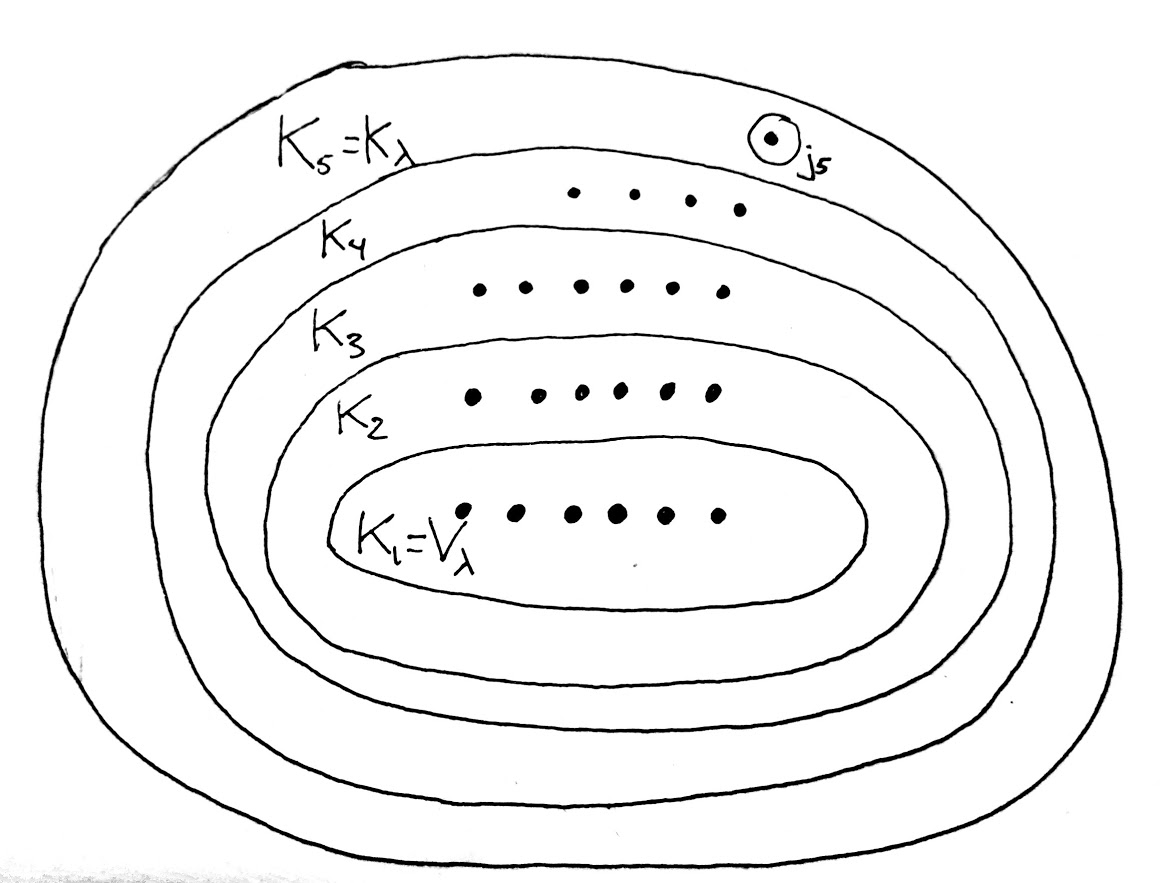
\includegraphics[width=\textwidth]{basis}
	\end{minipage}
	\begin{minipage}{0.5\textwidth}
	$j_r = \B j_{r+1}\\
	j_{r+1} \in K_{r+1} = Ker \B^{r+1} = Ker(\A - \lambda\E)^{r+1}\n
	\B^r j_r = \B ^r \B j_{r+1} = \B ^{r+1} j _{r+1} = \0 \n
	\Rightarrow j_r \ in K_r = Ker \B^r\n
	L = span(j_1 \ j_2 \ j_3 \ j_4 \ j_5)\n$
	\end{minipage}\n
	$\A|_{L}\n
	\begin{array}{ccccc}
		\begin{pmatrix}
			\lambda\\
			0\\0\\0\\0
		\end{pmatrix}
		& \begin{pmatrix}
		1\\
		\lambda\\
		0\\0\\0
		\end{pmatrix}
		& \begin{pmatrix}
		0\\1\\
		\lambda\\
		0\\0
		\end{pmatrix}
		& \begin{pmatrix}
		0\\0\\1\\
		\lambda\\
		0
		\end{pmatrix}
		& \begin{pmatrix}
		0\\0\\0\\1\\
		\lambda
		\end{pmatrix}\\
		\updownarrow & \updownarrow &\updownarrow &\updownarrow &\updownarrow\\
		\A j_1 = \lambda j_1 &
		\A j_2 = j_1 + \lambda j_2 &
		\A j_3 = j_2 + \lambda j_3 &
		\A j_4 = j_3 + \lambda j_4 &
		\A j_5 = j_4 + \lambda j_5
	\end{array}\n
	\text{Матрица }\A|_L \text{ в базисе } j = A_j = \begin{pmatrix}
		\lambda & 1 & 0 & 0 & 0\\
		0 & \lambda & 1 & 0 & 0\\
		0 & 0 & \lambda & 1 & 0\\
		0 & 0 & 0 & \lambda & 1\\
		0 & 0 & 0 & 0 & \lambda
	\end{pmatrix}$ $\begin{matrix}\text{\textbf{Клетка Жордана }} \boldsymbol{5\times 5}\\
		\text{(блок нижнего уровня)}
		\end{matrix}\n
	(j_5\ j_4 \ j_3 \ j_2 \ j_1) \rightarrow \begin{pmatrix}
		\lambda & \ldots & \ldots & 0\\
		1 & \ddots & & \vdots\\
		\vdots & \ddots & \ddots & \vdots\\
		0 & \ldots & 1 & \lambda
	\end{pmatrix}$\n
	\begin{minipage}{0.5\textwidth}
		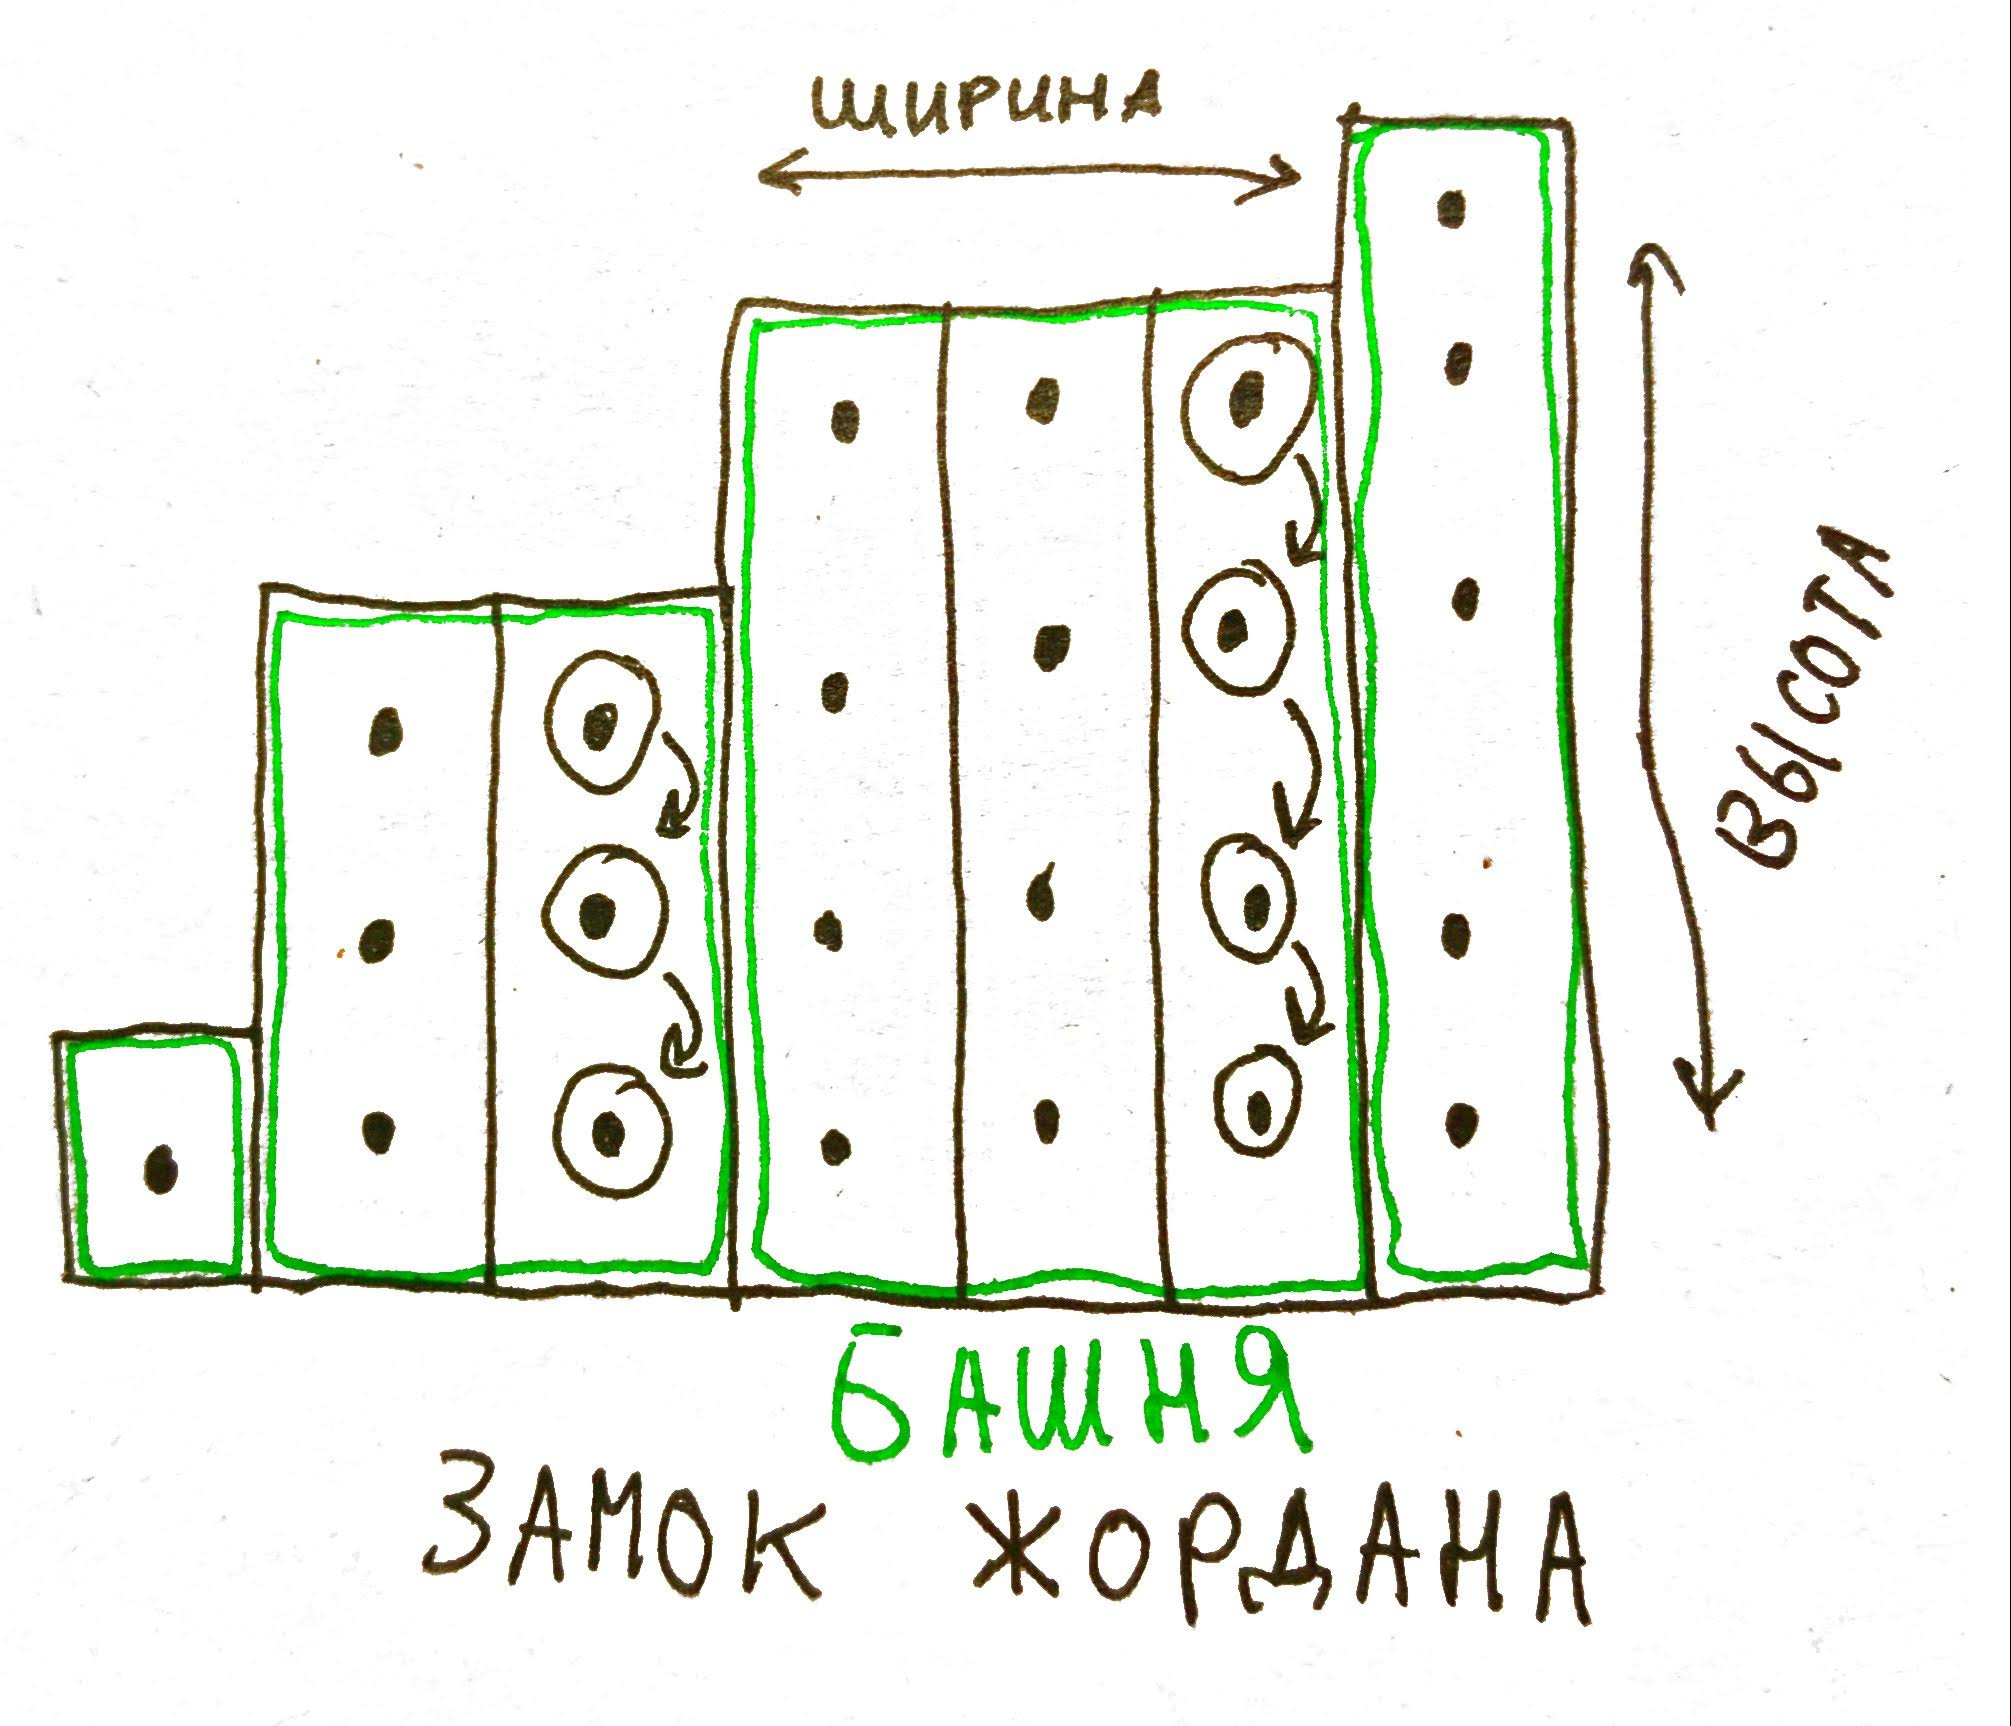
\includegraphics[width=\textwidth]{castle}
	\end{minipage}
	\begin{minipage}{0.5\textwidth}
		\textbf{Башня} -- циклическое объединение базисов одной длины.\\
		\textbf{Высота башни} -- количество векторов в базисе.\\
		\textbf{Ширина башни} -- число циклических базисов одной размерности\\
		\textbf{Основания} каждой башни в собственном подпространстве\\
		Число циклических базисов = $\gamma$\\
		$\slide{0.2in}||$\\
		Число Жордановых клеток
	\end{minipage}\n
	$
	\begin{matrix}\begin{pmatrix}
		\boxed{\lambda}\\
		& \boxed{\begin{matrix}
			\boxed{\begin{matrix}
					\lambda & 1\\
					& \lambda & 1\\
					& & \lambda
				\end{matrix}} &  \leftarrow \begin{array}{l}\text{Блок}\\ \text{нижнего}\\ \text{уровня}\end{array}\\
			& \boxed{\begin{matrix}
				\lambda & 1\\
				& \lambda & 1\\
				& & \lambda
				\end{matrix}}
			\end{matrix}}\\
		& \begin{array}{r}
			\text{Блок среднего}\\
			\text{уровня}\\
			\text{(отвечает башне)}
		\end{array} \rightarrow & \boxed{\begin{matrix}
				\boxed{\begin{matrix}
						\lambda & 1\\
						& \lambda & 1\\
						& & \lambda & 1\\
						& & & \lambda
					\end{matrix}} \\
				& \boxed{\begin{matrix}
					\lambda & 1\\
					& \lambda & 1\\
					& & \lambda & 1\\
					& & & \lambda
					\end{matrix}}\\
				& & \boxed{\begin{matrix}
					\lambda & 1\\
					& \lambda & 1\\
					& & \lambda & 1\\
					& & & \lambda
					\end{matrix}}
			\end{matrix}}\\
		& & & \boxed{\begin{matrix}
				\lambda & 1\\
				& \lambda & 1\\
				& & \lambda & 1\\
				& & & \lambda & 1\\
				& & & & \lambda
			\end{matrix}}
	\end{pmatrix}\\
	\overset{\uparrow}{\text{Блок верхнего уровня, отвечает }K_\lambda}
	\end{matrix}$\n
	$\gamma = $ Число блоков нижнего уровня\\
	$\alpha = $ Число $\lambda$ на диагонали\n
	$\A $ о.п.с. $\forall \alpha = \gamma\\
	V_\lambda \; \; \boxed \cdot \ \boxed \cdot\ \boxed \cdot \ \boxed \cdot \ \boxed \cdot$\\
	"Деревня Жордана" 
\end{document}